\subsection{Further Work}
While GKAGE demonstrates that alignment-free genotyping can be sped up through GPU acceleration, we believe that the current GKAGE runtimes can still be significantly improved.
We will here identify some possible avenues where the current implementation can be altered or improved in order to better use the hardware and technology available to gain more speedup.

\subsubsection{Better GPU Hash Table}
While the GPU hash table used in GKAGE for \textit{k}mer counting is plenty effective for our purpose of demonstrating the effectiveness of GPU acceleration in alignment-free genotyping, alternative hash tables exist that, with correct integration, should perform better.
Since optimizing GPU hash tables is all but a dicipline in and of itself and beyond the scope of this thesis, our GPU hash table implements a naive solution for collision handling and probing.
An interesting future avenue would be to integrate a version a bucketed static cuckoo hash table from BGHT \cite{bght} to evaluate how a state-of-the-art hash table would perform compared to our own.
Although faster, we doubt the effect would be dramatic in our case.

\subsubsection{Parallelization of \textit{k}mer Chunk Preparation}
Recall that in the \textit{k}mer counting step in KAGE, the input FASTA file is read in chunks.
Each chunk of data is then 2-bit encoded and all valid \textit{k}mers are hashed from the 2-bit encoded data chunk.
Finally, the chunk of hashed \textit{k}mers are counted.
In GKAGE, the 2-bit encoding, \textit{k}mer hashing and \textit{k}mer counting are performed on the GPU.
Thus, the chunk of data read from the FASTA file is copied to the GPU's memory before processing begins.
Currently, GKAGE performs all of these processes sequentially.

\vspace{.5em}
\begin{figure}[H]
\begin{center}
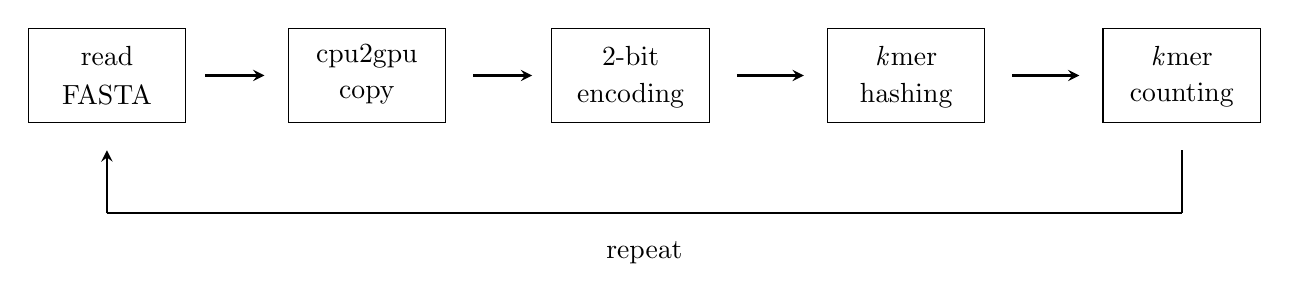
\begin{tikzpicture}
  % read fasta
  \node at(0,0)[draw,minimum width=2cm,minimum height=1.2cm](start){};
  \node at(0,.25)[]{\smaller{read}};
  \node at(0,-.25)[]{\smaller{FASTA}};
  \draw [thick,-stealth](1.25,0) -- (2,0);
  % cpu2gpu copy
  \node at(3.3,0)[draw,minimum width=2cm,minimum height=1.2cm]{};
  \node at(3.3,.25)[]{\smaller{cpu2gpu}};
  \node at(3.3,-.25)[]{\smaller{copy}};
  \draw [thick,-stealth](4.65,0) -- (5.4,0);
  % 2-bit encoding
  \node at(6.65,0)[draw,minimum width=2cm,minimum height=1.2cm]{};
  \node at(6.65,.25)[]{\smaller{2-bit}};
  \node at(6.65,-.25)[]{\smaller{encoding}};
  \draw [thick,-stealth](8,0) -- (8.85,0);
  % kmer hashing
  \node at(10.15,0)[draw,minimum width=2cm,minimum height=1.2cm]{};
  \node at(10.15,.25)[]{\smaller{\textit{k}mer}};
  \node at(10.15,-.25)[]{\smaller{hashing}};
  \draw [thick,-stealth](11.50,0) -- (12.35,0);
  % kmer counting
  \node at(13.65,0)[draw,minimum width=2cm,minimum height=1.2cm](end){};
  \node at(13.65,.25)[]{\smaller{\textit{k}mer}};
  \node at(13.65,-.25)[]{\smaller{counting}};
  % arrows
  \draw [thick](13.65,-.95) -- (13.65,-1.75);
  \draw [thick](13.65,-1.75) -- (0,-1.75);
  \draw [thick,-stealth](0,-1.75) -- (0,-.95);
  \node at(6.825,-2.25)[]{\smaller{repeat}};
\end{tikzpicture}
\caption{
  GKAGE's current \textit{k}mer counting pipeline performs several steps in a sequential fashion.
  While these steps are performed on many \textit{k}mers in parallel at once, each chunk (containing many \textit{k}mers) is processed sequentally. 
}
\label{discussion:parallelization_of_kmer_chunk_preparation:figures:pipeline}
\end{center}
\end{figure}

By utilizing CUDA streams we can parallelize the copying of data to the GPU and the processing of the previous chunk, creating a new and more efficient pipeline.

\begin{figure}[H]
\begin{center}
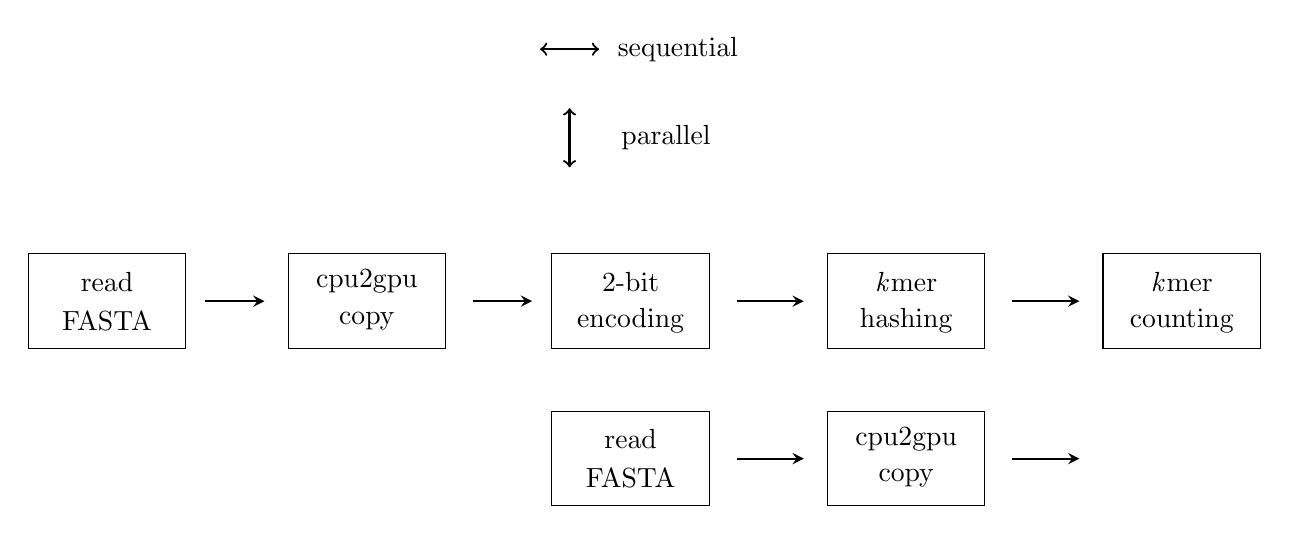
\begin{tikzpicture}
  % hints
  \draw [thick,<->](5.875,2.45) -- (5.875,1.7);
  \node at(7.1,2.075)[]{\smaller{parallel}};
  \draw [thick,<->](5.5,3.2) -- (6.25,3.2);
  \node at(7.25,3.2)[]{\smaller{sequential}};
  % read fasta
  \node at(0,0)[draw,minimum width=2cm,minimum height=1.2cm](start){};
  \node at(0,.25)[]{\smaller{read}};
  \node at(0,-.25)[]{\smaller{FASTA}};
  \draw [thick,-stealth](1.25,0) -- (2,0);
  % cpu2gpu copy
  \node at(3.3,0)[draw,minimum width=2cm,minimum height=1.2cm]{};
  \node at(3.3,.25)[]{\smaller{cpu2gpu}};
  \node at(3.3,-.25)[]{\smaller{copy}};
  \draw [thick,-stealth](4.65,0) -- (5.4,0);
  % 2-bit encoding
  \node at(6.65,0)[draw,minimum width=2cm,minimum height=1.2cm]{};
  \node at(6.65,.25)[]{\smaller{2-bit}};
  \node at(6.65,-.25)[]{\smaller{encoding}};
  \draw [thick,-stealth](8,0) -- (8.85,0);
  % kmer hashing
  \node at(10.15,0)[draw,minimum width=2cm,minimum height=1.2cm]{};
  \node at(10.15,.25)[]{\smaller{\textit{k}mer}};
  \node at(10.15,-.25)[]{\smaller{hashing}};
  \draw [thick,-stealth](11.5,0) -- (12.35,0);
  % kmer counting
  \node at(13.65,0)[draw,minimum width=2cm,minimum height=1.2cm](end){};
  \node at(13.65,.25)[]{\smaller{\textit{k}mer}};
  \node at(13.65,-.25)[]{\smaller{counting}};
  % read fasta 2
  \node at(6.65,-2)[draw,minimum width=2cm,minimum height=1.2cm](start){};
  \node at(6.65,-1.75)[]{\smaller{read}};
  \node at(6.65,-2.25)[]{\smaller{FASTA}};
  \draw [thick,-stealth](8,-2) -- (8.85,-2);
  % cpu2gpu copy 2
  \node at(10.15,-2)[draw,minimum width=2cm,minimum height=1.2cm]{};
  \node at(10.15,-1.75)[]{\smaller{cpu2gpu}};
  \node at(10.15,-2.25)[]{\smaller{copy}};
  \draw [thick,-stealth](11.5,-2) -- (12.35,-2);
\end{tikzpicture}
\caption{
  An illustration of a more optimal \textit{k}mer counting pipeline.
  By utilizing CUDA's streams, we can parellalize copying of data to the GPU and actual GPU processing.
}
\label{discussion:parallelization_of_kmer_chunk_preparation:figures:parallel_pipeline}
\end{center}
\end{figure}
